\begin{blocksection}

\question
b)  The revised accumulator circuit has been modified below with a register.  At every rising edge of the clock, registers will take in new input and then output it at the other end.  Write the values of the output for time t = 0 through t = 3, given the register and input both held value 0 before time t = 0 and given the input stream 0x01, 0x5A, 0x00, and 0x13.

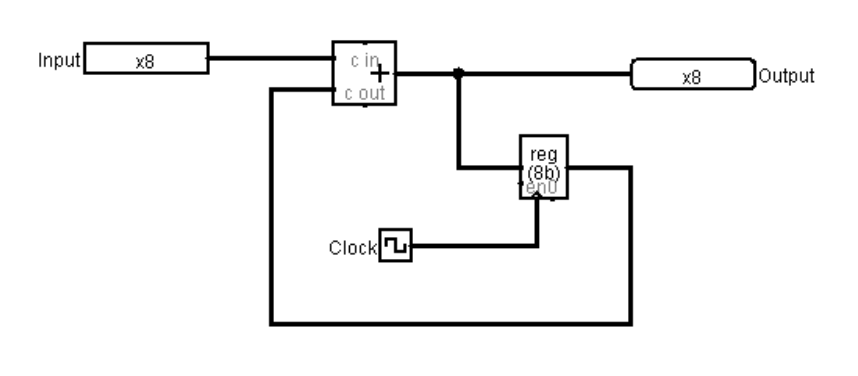
\includegraphics[width=\textwidth]{sds/registers_b}

\begin{tabular}{ |l|l|l|l|l| } 
 \hline
 Time: & t = 0 & t = 1 & t = 2 & t = 3 \\ 
 \hline
 Input: & 0x01 & 0x5A & 0x00 & 0x13 \\ 
 \hline
 Output: &  &  &  &  \\ 
 \hline
\end{tabular}

\begin{solution}
\begin{tabular}{ |l|l|l|l|l| } 
 \hline
 Time: & t = 0 & t = 1 & t = 2 & t = 3 \\ 
 \hline
 Input: & 0x01 & 0x5A & 0x00 & 0x13 \\ 
 \hline
 Output: & 0x01 & 0x5B & 0x5B & 0xBE \\ 
 \hline
\end{tabular}
\end{solution}

\end{blocksection}